% Appendix X

\chapter{User Defined Functions}

\definecolor{main-color}{rgb}{0.6627, 0.7176, 0.7764}
\definecolor{back-color}{rgb}{0.1686, 0.1686, 0.1686}
\definecolor{string-color}{rgb}{0.3333, 0.5254, 0.345}
\definecolor{key-color}{rgb}{0.8, 0.47, 0.196}
\definecolor{myblue}{rgb}{0.117647 0.564706 1}
\definecolor{codegreen}{rgb}{0,0.6,0}


\lstdefinestyle{mystyle}{
	language = SQL,
	basicstyle = {\color{main-color}},
	backgroundcolor = {\color{back-color}},
	commentstyle=\color{codegreen},
	stringstyle = {\color{string-color}},
	keywordstyle = {\color{key-color}},
	keywordstyle = [2]{\color{red}},
	keywordstyle = [3]{\color{teal}},
	keywordstyle = [4]{\color{myblue}},
	otherkeywords = {PER, PERFORM, REPLACE, function, returns, void, DECLARE, BEGIN, LOOP, IF, FOR, LANGUAGE, FUNCTION, RETURNS, TEMP, TRUNCATE, WHILE, if},
	morekeywords = [2]{RECORD, geometry, SERIAL},
	morekeywords = [3]{\$\$},
	morekeywords = [4]{ST_Intersects, ST_Intersection, ST_Buffer, st_intersection, st_geometrytype, st_dump, st_linemerge, st_collectionextract, st_split, st_area, ST_Perimeter, st_centroid, st_x, st_y, regr_slope, st_makepoint, st_makeline, st_setsrid, st_distance, ST_LineSubString, st_lineinterpolatepoint, st_length},
	numberstyle=\normalfont\footnotesize\color{black},
	stepnumber=1,
	tabsize=2,
	literate=
	{á}{{\'a}}1 {é}{{\'e}}1 {í}{{\'i}}1 {ó}{{\'o}}1 {ú}{{\'u}}1
	{Á}{{\'A}}1 {É}{{\'E}}1 {Í}{{\'I}}1 {Ó}{{\'O}}1 {Ú}{{\'U}}1
	{à}{{\`a}}1 {è}{{\`e}}1 {ì}{{\`i}}1 {ò}{{\`o}}1 {ù}{{\`u}}1
	{À}{{\`A}}1 {È}{{\'E}}1 {Ì}{{\`I}}1 {Ò}{{\`O}}1 {Ù}{{\`U}}1
	{ä}{{\"a}}1 {ë}{{\"e}}1 {ï}{{\"i}}1 {ö}{{\"o}}1 {ü}{{\"u}}1
	{Ä}{{\"A}}1 {Ë}{{\"E}}1 {Ï}{{\"I}}1 {Ö}{{\"O}}1 {Ü}{{\"U}}1
	{â}{{\^a}}1 {ê}{{\^e}}1 {î}{{\^i}}1 {ô}{{\^o}}1 {û}{{\^u}}1
	{Â}{{\^A}}1 {Ê}{{\^E}}1 {Î}{{\^I}}1 {Ô}{{\^O}}1 {Û}{{\^U}}1
	{œ}{{\oe}}1 {Œ}{{\OE}}1 {æ}{{\ae}}1 {Æ}{{\AE}}1 {ß}{{\ss}}1
	{ű}{{\H{u}}}1 {Ű}{{\H{U}}}1 {ő}{{\H{o}}}1 {Ő}{{\H{O}}}1
	{ç}{{\c c}}1 {Ç}{{\c C}}1 {ø}{{\o}}1 {å}{{\r a}}1 {Å}{{\r A}}1
	{€}{{\euro}}1 {£}{{\pounds}}1 {«}{{\guillemotleft}}1
	{»}{{\guillemotright}}1 {ñ}{{\~n}}1 {Ñ}{{\~N}}1 {¿}{{?`}}1
}

In questo capitolo vengono illustrate le User Defined Functions (da qui in avanti indicate con l’acronimo UDFs), per il calcolo del valore di exposure per le stazioni ferroviarie nonché per le linee ferroviarie. Tali UDFs sono state realizzate nel linguaggio PL/pgSQL offerto da PostgreSQL, sfruttando le funzioni fornite dall’estensione spaziale PostGIS.

\section{UDFs per le stazioni}
E' stato realizzato uno script Python, \textit{HotSpotCalculator}, in grado di collegarsi al database ed eseguire la UDF  \textit{\_\_Exposure(id\_point)}. Quest'ultima è la funzione fondamentale in quanto richiama sequenzialmente tutte le UDF necessarie per il calcolo dell'exposure di una stazione. L'ultima UDF eseguita, ovvero la \textit{\_\_ContributionOfLandslide(id\_point,l)} inserisce il risultato nella tabella \textit{exposure\_station}.
Lo script Python itera \textit{\_\_Exposure} per tutte le stazioni (Figura \ref{diagramma_algoritmo}).  

\begin{figure}[h]
	\centering
	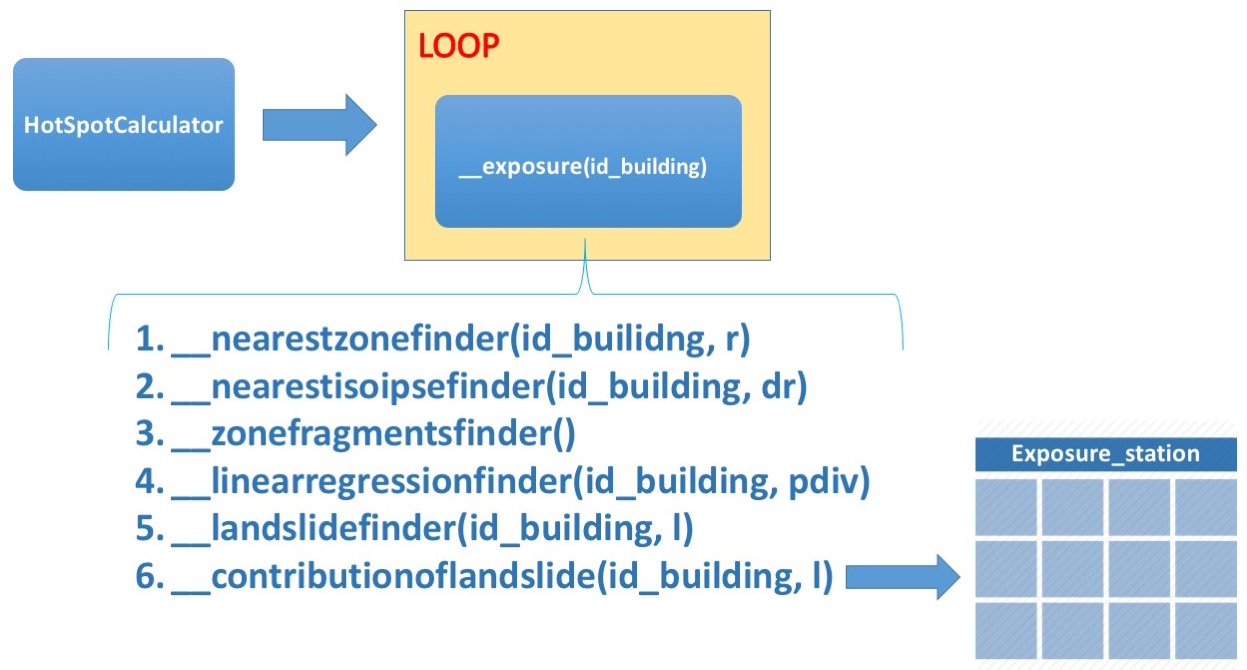
\includegraphics[width=0.9\textwidth]{images/algorithm}
	\caption{Diagramma del funzionamento dell'algoritmo realizzato.}
	\label{diagramma_algoritmo}
\end{figure}

Inoltre stima il tempo necessario al completamento dei calcoli e fornisce lo stato di avanzamento delle operazioni inteso come il numero di stazioni per il quale è stato calcolato l'exposure rispetto al totale.ì .



\subsection{\_\_exposure}
\textbf{INPUT}: \textit{id\_point} generico punto sul quale si vuole calcolare l'exposure. In questo caso di studio corrisponde all'ID del $b_i$.\newline
\textbf{OUTPUT}: \textit{void}. \newline
\textbf{COMMENTO}: Rappresenta la main function. Esegue in successione sulla $b_i$ le UDF necessarie al calcolo dell'exposure. Crea la tabella exposure\_stations dove verranno salvato il valore dell'exposure.   

\small
\begin{lstlisting}[style = mystyle]
create or REPLACE function "__exposure"(id_point integer) returns void
LANGUAGE plpgsql
AS $$
DECLARE
	point RECORD;
	exposure RECORD;
BEGIN
	
	-- Reset delle tabelle di appoggio.
	DROP TABLE IF EXISTS nearestzones;
	DROP TABLE IF EXISTS nearestisoipses;
	DROP TABLE IF EXISTS zonefragments;
	DROP TABLE IF EXISTS linearregression;
	DROP TABLE IF EXISTS hazardzones;
	DROP TABLE IF EXISTS landslide;
	DROP TABLE IF EXISTS exposure_stations;
	
	-- Creazione della tabella dove veranno inseriti i risultati finali delle exposure
	CREATE TABLE IF NOT EXISTS exposure_stations (
		Building_gid INTEGER PRIMARY KEY REFERENCES railway_stations(gid),
		exposure FLOAT
	);

	DROP TABLE IF EXISTS points;
	CREATE TABLE points AS (SELECT * FROM railway_stations);

	-- Esegue tutte le UDF per il calcolo dell'exposure sul generico punto.
	FOR point IN SELECT * FROM points where gid=id_point LOOP
		PERFORM __nearestzonefinder(point.gid,800);
		PERFORM __nearestisoipsefinder(point.gid,850);
		PERFORM __zonefragmentsfinder();
		PERFORM __linearregressionfinder(point.gid,2.5);
		PERFORM __landslidefinder(point.gid,50);
		PERFORM __contributionoflandslide(point.gid,50);

	SELECT * FROM exposure LIMIT 1 INTO exposure;
	
	--Memorizza il risultato del calcolo dell'exposure
	INSERT INTO exposure_stations (Building_gid, exposure) 
				VALUES (exposure.id, exposure.exposure);
	END LOOP;

	PERFORM __cleartables();
END;
$$;
\end{lstlisting}

\newpage
\subsection{\_\_NearestZoneFinder}
\textbf{INPUT}: 
\begin{enumerate}
	\item \textit{id\_point} è l'ID del $b_i$;
	\item \textit{r} è il raggio della $HazardArea_i$.
\end{enumerate}
\textbf{OUTPUT}: \textit{void}. \newline
\textbf{COMMENTO}: trova tutte le zone che si trovano all'interno della $HazardArea_i$ di $b_i$. I risultati vengo salvati all'interno della tabella NearestZones.

\small
\begin{lstlisting}[style = mystyle]
CREATE OR REPLACE FUNCTION "__nearestzonefinder"(id_point integer, r integer) returns void
LANGUAGE plpgsql
AS $$
DECLARE
	station RECORD;
	particella RECORD;
	hazardArea geometry;
BEGIN
	
	--Crea la tabella temporanea di appoggio per i risultati
	CREATE TEMP TABLE hotspottmp ( 
		id serial PRIMARY KEY, id_station INTEGER, geom Geometry, szk FLOAT  ) 
		ON COMMIT DROP;
	
	--Seleziona la stazione che si vuole analizzare
	SELECT * INTO station FROM points where gid = id_point;
	
	--Crea il buffer intorno alla stazione
	hazardArea := (SELECT ST_Buffer(station.geom, r));
	
	--Controlla queli zk (particella) cadono all'interno del buffer 
	--e aggiungila alla tabella temporanea. Se la zk non cade 
	--per intera nel buffer allora prendi l'intersezione.
	FOR particella IN SELECT * FROM zones LOOP
		IF ST_Intersects(hazardArea, particella.geom) THEN
			INSERT INTO hotspottmp (id_station, geom, szk) VALUES(
						station.gid, 
						ST_Intersection(hazardArea, particella.geom),
						particella.szk);
		END IF;
	END LOOP;
	
	--Copia i dati della tabella temporanea nella tabella NearestZones
	CREATE TABLE NearestZones AS SELECT * FROM hotspottmp;
	DROP TABLE hotspottmp;

END;
$$;

\end{lstlisting}

\subsection{\_\_NearestIsoipseFinder}

\textbf{INPUT}: 
\begin{enumerate}
	\item \textit{id\_point} è l'ID del $b_i$;
	\item \textit{dr} il raggio leggermente più grande rispetto all'$HazardArea_i$.
\end{enumerate}
\textbf{OUTPUT}: \textit{void}. \newline
\textbf{COMMENTO}: trova tutte le $ni_{i,o}$ e le inserisce nella tabella \textit{NearestIsoipses}. L'$HazardArea_i$ ha, in questo unico caso, un raggio leggermente più grande. Ciò è necessario per ottenere che le $ni_{i,o}$ escano dal perimetro delle $nz_{i,j}$ così che la UDF successiva (\textit{\_\_ZoneFragmentsFinder}) esegua correttamente la funzione ST\_SPLIT(). 

\begin{lstlisting}[style = mystyle]
CREATE OR REPLACE FUNCTION "__nearestisoipsefinder"(id_point integer, dr integer) returns void
LANGUAGE plpgsql
AS $$
DECLARE
	station RECORD;
	hazardArea geometry;
BEGIN
	
	--- Crea la tabella temporanea di appoggio per i dati
	CREATE TEMP TABLE tempIsoipse (
		id SERIAL PRIMARY KEY ,
		geom GEOMETRY,
		elevation INTEGER
	);
	
	--- Seleziona la stazione 
	SELECT * INTO station FROM points WHERE gid=id_point;
	
	--- Crea il buffer intorno alla stazione
	hazardArea := (SELECT ST_Buffer(station.geom, dr));

	--- Di tutte le curve di livello inserisce nella tabella 
	--- temporanea solo la parte che interseca il buffer 
	INSERT INTO tempIsoipse (elevation,geom) (
		SELECT
			isoipse_abruzzo_25.elevation,
			st_intersection(isoipse_abruzzo_25.geom,hazardArea) as geom
		FROM isoipse_abruzzo_25 
		WHERE st_intersects(isoipse_abruzzo_25.geom,hazardArea)
	);

	--- Elimina dalla tabella temporanea le geometrie di tipo 
	--- ST_MultiLineString. Sono inperfezioni che emergono nel 
	--- quando, nella istruzione precendente, 
	--- viene eseguita la della ST_intersects
	INSERT INTO tempIsoipse(elevation,geom) (
		SELECT 
			tempIsoipse.elevation,
			(st_dump(tempIsoipse.geom)).geom 
		FROM tempIsoipse 
		WHERE st_geometrytype(tempIsoipse.geom) = 'ST_MultiLineString');
		
	INSERT INTO tempIsoipse(elevation,geom) (
	SELECT 
		tempIsoipse.elevation, 
		st_linemerge(tempIsoipse.geom) 
	FROM tempIsoipse 
	WHERE st_geometrytype(tempIsoipse.geom) = 'ST_MultiLineString');

	DELETE FROM tempIsoipse WHERE st_geometrytype(tempIsoipse.geom) = 'ST_MultiLineString';


	CREATE TABLE NearestIsoipses AS SELECT * FROM tempIsoipse;

	DROP TABLE tempIsoipse;
END;
$$;
\end{lstlisting}

\subsection{\_\_ZoneFragmentsFinder}
\textbf{INPUT}: non ci sono parametri in ingresso. \newline
\textbf{OUTPUT}: \textit{void}. \newline
\textbf{COMMENTO}: suddivide tutti le $nz_{i,j}$ di $b_i$ in zone fragments. I risultati vengono inseriti nella tabella \textit{ZoneFragments}.

\begin{lstlisting}[style = mystyle]
CREATE OR REPLACE FUNCTION "__zonefragmentsfinder"() returns void
LANGUAGE plpgsql
AS $$
DECLARE
	NearestZone RECORD;
	PrimaIsoipse RECORD ;
	TempFragment RECORD;
	CurrentIsoipse RECORD;
	zoneCorrente RECORD;
BEGIN

	CREATE TABLE ZoneFragments(
		id SERIAL PRIMARY KEY ,
		geom GEOMETRY,
		id_zone INTEGER
	);

	--- Prende un primo poligono e lo interseca con le curve di livello
	--- risultanti dall'intersezione con il buffer già calcolate nell'UDF precedente.

	FOR NearestZone IN (SELECT * FROM  nearestzones) LOOP
		CREATE TEMP TABLE TempIsoipses(
			id INTEGER,
			geom GEOMETRY,
			elevation INTEGER
		);
		
		CREATE TEMP TABLE TempFragments(
			id SERIAL PRIMARY KEY ,
			geom GEOMETRY,
			id_zone INTEGER
		);
		CREATE TEMP TABLE CurrentIsoipses(
			id INTEGER ,
			geom GEOMETRY,
			elevation INTEGER
		);
		
		--- Prende una curva di livello
		SELECT * INTO zoneCorrente FROM nearestzones WHERE id = NearestZone.id;
		
		INSERT INTO TempIsoipses(id,geom,elevation) (
			SELECT
				nearestisoipses.id,
				(st_dump(st_collectionextract(st_intersection(nearestisoipses.geom,zoneCorrente.geom),2))).geom as geom,
				nearestisoipses.elevation 
			FROM nearestisoipses
		);

		--- Esegue la prima split tra la nearest zone e la curva di livello.
		SELECT * INTO PrimaIsoipse 
		FROM (
			SELECT * FROM nearestisoipses 
			WHERE (
				SELECT id From TempIsoipses LIMIT 1
			) = nearestisoipses.id) as prima;
	
		INSERT INTO TempFragments(geom,id_zone) (
			SELECT(
				st_dump(st_collectionextract(st_split(zoneCorrente.geom,PrimaIsoipse.geom),3))).geom , 
				zoneCorrente.id);
		
		--- Cancella la curva di livello in quanto è stata utilizzata 
		--- per lo split
		DELETE FROM TempIsoipses WHERE TempIsoipses.id = PrimaIsoipse.id;

		--- Esegue gli stessi passi precedenti (riga 42-61)
		--- su tutti i TempFragments 
		WHILE (SELECT count(*) FROM TempFragments) > 0 LOOP
			SELECT * INTO TempFragment FROM TempFragments LIMIT 1;
			INSERT INTO CurrentIsoipses(id,geom,elevation) (
				SELECT 				
					TempIsoipses.id,
					(st_dump(st_collectionextract(st_intersection(TempIsoipses.geom,TempFragment.geom),2))).geom as geom,
					TempIsoipses.elevation FROM TempIsoipses
				);
			IF (SELECT count(*) FROM CurrentIsoipses) > 0 THEN
				SELECT * INTO CurrentIsoipse FROM (
					SELECT * FROM nearestisoipses WHERE (
						SELECT id From CurrentIsoipses LIMIT 1) = nearestisoipses.id) as currentiso;
				
				INSERT INTO TempFragments(geom,id_zone) (
				SELECT(
					st_dump(st_collectionextract(st_split(TempFragment.geom,CurrentIsoipse.geom),3))).geom, zoneCorrente.id
				);
				
				--- Elimina la curva di livello utilizzata per la split
				DELETE FROM TempIsoipses WHERE TempIsoipses.id = CurrentIsoipse.id;
				
				--- Elimina la geometria di zk che è stata splittata ulterioremente.
				DELETE FROM TempFragments WHERE TempFragments.id = TempFragment.id;
			ELSE
				--- Il frammento non è più divisibile quindi viene inserito nella tabella ZoneFragments
				INSERT INTO ZoneFragments(geom,id_zone) VALUES (TempFragment.geom,TempFragment.id_zone);
				
				--- Il frammento non è più divisibile quindi viene eliminato dalla tabella temporanea.
				DELETE FROM TempFragments WHERE TempFragments.id = TempFragment.id;
			END IF;
			
			TRUNCATE TABLE CurrentIsoipses;
		END LOOP;

		DROP TABLE IF EXISTS TempIsoipses;
		DROP TABLE IF EXISTS TempFragments;
		DROP TABLE IF EXISTS CurrentIsoipses;
	END LOOP ;
	
	DELETE FROM ZoneFragments WHERE st_area(ZoneFragments.geom) < 100;
END;
$$;

\end{lstlisting}

\newpage
\subsection{\_\_linearregressionfinder}
\textbf{INPUT}: \textit{pdiv} parametro necessario per la costruzione della $blr_{i,j}$. \newline
\textbf{OUTPUT}: \textit{void}. \newline
\textbf{COMMENTO}: trova tutte le $blr_{i,j}$ che partono dalle nearest zones.

\begin{lstlisting}[style = mystyle]
CREATE OR REPLACE FUNCTION "__linearregressionfinder"(pdiv double precision) returns void
LANGUAGE plpgsql
AS $$
DECLARE
	x DOUBLE PRECISION;
	y DOUBLE PRECISION;
	xp DOUBLE PRECISION;
	yp DOUBLE PRECISION;
	slope DOUBLE PRECISION;
	id_zone_var INTEGER;
	line_buffer_size FLOAT;
BEGIN

	CREATE TABLE LinearRegression (
		id SERIAL,
		geom geometry,
		id_zone INTEGER
	);
	
	--- Per ogni nearest zone calcola la retta di regressione lineare
	FOR id_zone_var IN SELECT id FROM nearestzones LOOP

		DROP TABLE IF EXISTS point;
		DROP TABLE IF EXISTS Centroid_zone;
		DROP TABLE IF EXISTS slope_table;
		DROP TABLE IF EXISTS centroid_zoneFragments;

		CREATE TEMP TABLE point(
			geom GEOMETRY
		);

		CREATE TEMP TABLE Centroid_zone (
			id SERIAL,
			id_zone INTEGER,
			st_centroid geometry
		);
		
		--- Calcola il centro di massa della nearest zone
		INSERT INTO Centroid_zone(id_zone, st_centroid) 
			SELECT 
				id, 
				st_centroid(nearestzones.geom) 
			FROM nearestzones;

		xp := (
			SELECT st_x(Centroid_zone.st_centroid) 
			FROM Centroid_zone 
			WHERE Centroid_zone.id_zone = id_zone_var
		);
		
		yp := (
			SELECT st_y(Centroid_zone.st_centroid) 
			FROM Centroid_zone 
			WHERE Centroid_zone.id_zone = id_zone_var);

		CREATE TEMP TABLE centroid_zoneFragments(
			id SERIAL,
			centroid_fragments geometry
		);

		--- Calcola i centri di massa degli zone fragments della nearest zone
		INSERT INTO centroid_zoneFragments(centroid_fragments) 
			SELECT st_centroid(geom) 
			FROM zonefragments 
			WHERE id_zone = id_zone_var;

		CREATE TABLE slope_table AS (
			SELECT 
				st_x(centroid_zoneFragments.centroid_fragments) as x_slope, st_y(centroid_zoneFragments.centroid_fragments) as y_slope 
			FROM centroid_zoneFragments
		);
		
		--- Utilizza i centri di massa per calcolare il coefficente angolare
		--- della retta di regressione lineare
		SELECT regr_slope(slope_table.y_slope, slope_table.x_slope) 
		INTO slope 
		FROM slope_table;
	
		--SELECT (AVG(ST_Perimeter(geom)))/pdiv INTO line_buffer_size FROM zonefragments WHERE id_zone = id_zone_var;
	
		SELECT (ST_Perimeter(geom))/pdiv 
		INTO line_buffer_size 
		FROM nearestzones 
		WHERE id = id_zone_var;

		x:= 2503811;
		y:= yp + slope*(x - xp);

		INSERT INTO point SELECT st_makepoint(x,y);

		x:= 2354956;
		y:= yp + slope*(x - xp);

		INSERT INTO point SELECT st_makepoint(x,y);
		
		--- controlla se ci sono almeno 3 centri di massa 
		--- altrimenti non ha senso calcolare la retta di regressione lineare
		IF (SELECT count(centroid_zoneFragments.centroid_fragments) 
			FROM centroid_zoneFragments) > 3 THEN
			
				INSERT INTO LinearRegression(geom, id_zone)
				 VALUES ((
				 	SELECT st_buffer(st_makeline(st_setsrid(point.geom,3004)), line_buffer_size) 
				 	FROM point), 
				 id_zone_var
				 );
		END IF;
	END LOOP;
END;
$$;

\end{lstlisting}

\subsection{\_\_contributionoflandslide}
\textbf{INPUT}: 
\begin{enumerate}
	\item \textit{id\_point} è l'ID del $b_i$;
	\item \textit{l} raggio del $BuildingBuffer_i$.
\end{enumerate}
\textbf{OUTPUT}: \textit{void}. \newline
\textbf{COMMENTO}: trova tutte le $ls_{i,j}$ che impattano sulla stazione, ovvero che intersecano il $BuildingBuffer_i$

\begin{lstlisting}[style = mystyle]
CREATE OR REPLACE FUNCTION "__contributionoflandslide"(id_point integer, l double precision) returns void
LANGUAGE plpgsql
AS $$
DECLARE
	landslidezone RECORD;
	exposure FLOAT;
	CurrentPoint RECORD;
	avg_area FLOAT;
	impfact FLOAT;
	landslide GEOMETRY;
	distance FLOAT;
BEGIN

	CREATE TABLE IF NOT EXISTS exposure (
		id SERIAL PRIMARY KEY,
		point_gid real,
		exposure FLOAT
	);

	exposure := 0;
	
	SELECT * INTO CurrentPoint FROM points WHERE gid = id_point;
	SELECT avg(st_area(geom)) INTO avg_area FROM zones;
	
	--- Per ogni landslide controlla se interseca il building buffer.
	--- Se è vero allora la landslide contribusce all'exposure
	--- altrimenti no.
	FOR landslidezone IN (SELECT * FROM landslidezones) LOOP
		IF (ST_Intersects(CurrentPoint.geom, landslidezone.geom)) THEN
			exposure := exposure + (st_area(landslidezone.geom) * landslidezone.szk);
		ELSE
			distance:=st_distance(CurrentPoint.geom, landslidezone.geom);
			SELECT geom 
			INTO landslide 
			FROM linearregression 
			WHERE linearregression.id_zone = landslidezone.id;
		impfact :=
			(st_area(st_intersection(st_buffer(CurrentPoint.geom,l),landslide)))/
			(st_area(st_buffer(CurrentPoint.geom,l)));
		exposure := 
			(exposure + ((st_area(landslidezone.geom) * landslidezone.szk)*impfact));
		END IF;
	END LOOP;

	--INSERT INTO exposure (Building_gid, name, geom, exposure) VALUES (Building.gid, Building.name, Building.geom, exposure/avg_area);
	
	INSERT INTO exposure (point_gid, exposure) 
	VALUES (CurrentPoint.gid, exposure/avg_area);
END;
$$;
\end{lstlisting}

\newpage

\section{UDFs per le linee ferroviarie}

Lo script Python, \textit{HotSpotCalculatorRoutes} si collega al database ed esegue la UDF  \textit{\_\_exposure\_routes(id\_point)}. Quest'ultima è la funzione fondamentale in quanto richiama sequenzialmente tutte le UDF necessarie per il calcolo dell'exposure di una linea ferroviaria. L'ultima UDF eseguita, ovvero la \textit{\_\_contributionoflandslide(id\_point,l)} inserisce il risultato nella tabella \textit{exposure\_routes} (Figura \ref{diagramma_algoritmo2}).


\begin{figure}[h]
	\centering
	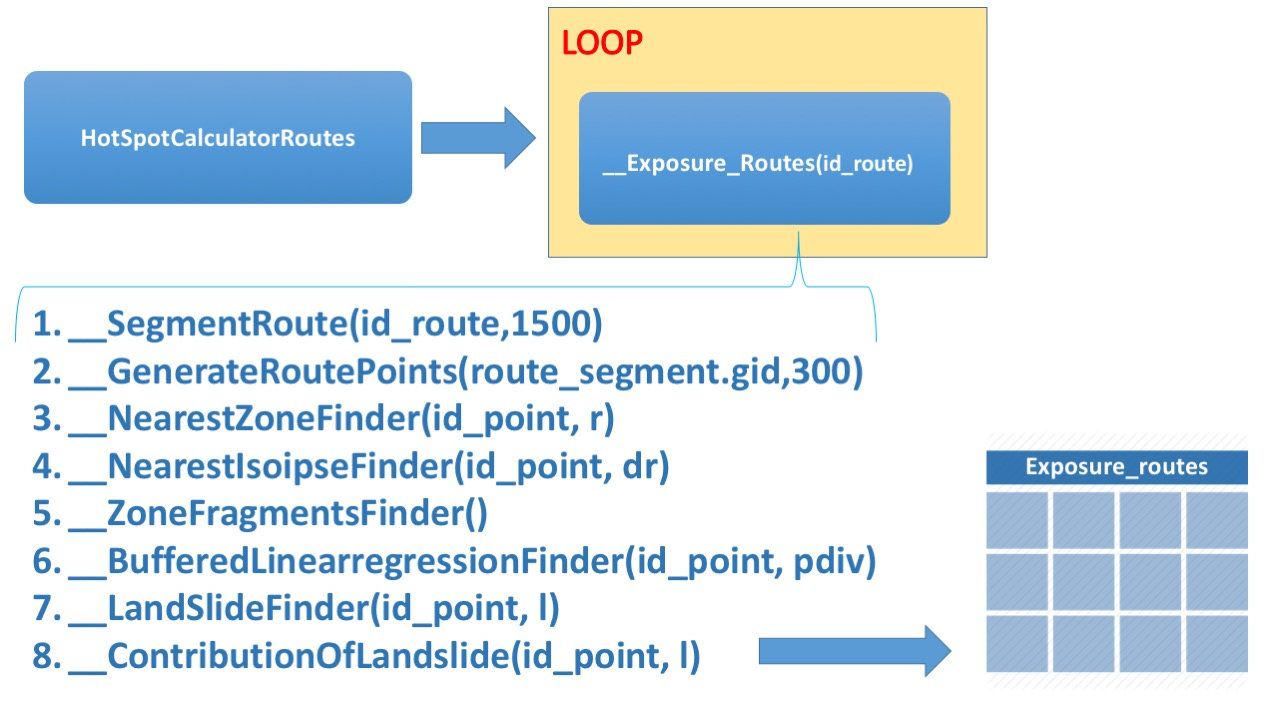
\includegraphics[width=0.9\textwidth]{images/algorithm2}
	\caption{Diagramma del funzionamento dell'algoritmo realizzato nel caso delle linee ferroviarie.}
	\label{diagramma_algoritmo2}
\end{figure}

\subsection{\_\_exposure\_routes}

\textbf{INPUT}: \textit{id\_route} è l'ID del $r_k$ \newline
\textbf{OUTPUT}: \textit{void}. \newline
\textbf{COMMENTO}: Rappresenta la main function. Esegue in successione sulle $r_K$ le UDF necessarie al calcolo dell’exposure. Crea la tabella exposure\_routes dove verranno salvato il valore dell’exposure.

\begin{lstlisting}[style = mystyle]
CREATE OR REPLACE function "__exposure_routes"(id_route integer) returns void
LANGUAGE plpgsql
AS $$
DECLARE
	point RECORD;
	route_segment RECORD;
	points INTEGER;
	iterator INTEGER;
	divisor INTEGER;
	lastexposure RECORD;
	startid INTEGER;
BEGIN

	DROP TABLE IF EXISTS current_route_segments;
	
	--- Richiama la funzione responsabile della suddivisione in sotto-tratte 
	PERFORM "__SegmentRoute"(id_route,1500);

	--- Su ogni sotto-tratta vengono campionati dei punti distanti tra loro 300 metri.
	FOR route_segment IN SELECT * FROM current_route_segments LOOP
		PERFORM "__GenerateRoutePoints"(route_segment.gid,300);
	END LOOP;

	DROP TABLE IF EXISTS points;
	CREATE TABLE  points AS (
		SELECT * 
		FROM current_route_points 
		ORDER BY gid ASC
	);
	
	DROP TABLE IF EXISTS current_route_points;

	SELECT COUNT(*) FROM points INTO points;
	SELECT COUNT(*) FROM points WHERE km=0 INTO divisor;
	SELECT gid FROM points LIMIT 1 INTO startid;
	
	iterator:=1;
	
	RAISE NOTICE 'TOTAL POINTS %',points;
	
	--- Per ciascun punto vengono richiamate le funzioni precedentemente utilizzate per il calcolo
	--- dell'exposure sulle stazioni.
	FOR point IN SELECT * FROM points LOOP
		RAISE NOTICE 'POINT NUMBER %',iterator;
		
		IF (point.gid-startid)%divisor=0 AND iterator!=1 THEN
			RAISE NOTICE 'JUMPED EXPOSURE %',iterator;
			SELECT * FROM exposure ORDER BY id DESC LIMIT 1 INTO lastexposure;

			--  SELECT gid FROM route_points WHERE route_points.geom=point.geom ORDER BY gid DESC LIMIT 1 INTO pointid;
			RAISE NOTICE 'ID POINT %',point.gid;
			--INSERT INTO exposure (building_gid, name, geom, exposure) VALUES (point.gid, point.name, point.geom, lastexposure.exposure);

			INSERT INTO exposure (point_gid, exposure) VALUES (point.gid, lastexposure.exposure);
		ELSE

			DROP TABLE IF EXISTS nearestzones;
			DROP TABLE IF EXISTS nearestisoipses;
			DROP TABLE IF EXISTS zonefragments;
			DROP TABLE IF EXISTS linearregression;
			DROP TABLE IF EXISTS landslidezones;
			DROP TABLE IF EXISTS landslide;
	
			PERFORM __nearestzonefinder(point.gid,800);
			PERFORM __nearestisoipsefinder(point.gid,850);
			PERFORM __zonefragmentsfinder();
			PERFORM __linearregressionfinder(point.gid,2.5);
			PERFORM __landslidefinder(point.gid,50);
			PERFORM __contributionoflandslide(point.gid,50);

		END IF;

		iterator:=iterator+1;

	END LOOP;

	CREATE TABLE IF NOT EXISTS exposure_route_points (
		pointid INTEGER PRIMARY KEY REFERENCES route_points(gid) ,
		exposure FLOAT
	);
	
	CREATE TABLE IF NOT EXISTS exposure_routes (
		routeid INTEGER PRIMARY KEY REFERENCES route_segments(gid),
		exposure FLOAT
	);

	INSERT INTO exposure_route_points (pointid,exposure) 
		SELECT point_gid,exposure FROM exposure;
	
	INSERT INTO exposure_routes (routeid,exposure) 
		SELECT t.gid, AVG(e.exposure) 
		FROM route_points as p INNER JOIN exposure as e ON p.gid=e.point_gid
		INNER JOIN route_segments as t ON t.gid=p.segmentid GROUP BY t.gid;

	PERFORM __cleartables();
END;
$$;

\end{lstlisting}

\subsection{\_\_SegmentRoute}

\textbf{INPUT}: 
\begin{enumerate}
	\item \textit{id\_route} è l'ID del $r_k$;
	\item \textit{step} lunghezza massima, in metri, di ciascuna sotto-tratta. 
\end{enumerate}
\textbf{OUTPUT}: \textit{void}. \newline
\textbf{COMMENTO}: suddivide le tratte in sotto-tratte $rs_{k,s}$.

\begin{lstlisting}[style = mystyle]
CREATE OR REPLACE FUNCTION "__SegmentRoute"(id_route integer, step integer) returns void
LANGUAGE plpgsql
AS $$
DECLARE
	route        RECORD;
	route_length FLOAT;
	divisore     INTEGER;
	passo        INTEGER;
	i            INTEGER;
	sts          FLOAT;
	ends         FLOAT;
	km           real;
	geome        GEOMETRY;
	line         RECORD;
BEGIN

	passo:=step;

	CREATE TABLE IF NOT EXISTS route_segments (
		gid   SERIAL PRIMARY KEY,
		route_id INTEGER REFERENCES railway_routes(gid),
		km   real,
		geom GEOMETRY
	);

	CREATE TABLE IF NOT EXISTS current_route_segments (
		gid   SERIAL PRIMARY KEY,
		km   real,
		geom GEOMETRY,
		name VARCHAR
	);
	
	
	SELECT
		id,
		st_linemerge(geom) AS geom,
		railway_routes.name
	INTO route
	FROM railway_routes
	WHERE id = id_route;
	
	--- Ottiene la lunghezza della route 
	route_length:=st_length(route.geom);
	
	--- La divide per il passo di segmentazione in questo modo
	--- conosce in anticipo il numero di sotto-tratte
	divisore:=route_length / passo;

	i:=0;
	
	--- Fin quando non finisco di suddividere la tratta eseguo
	--- il while
	WHILE i < divisore LOOP
		km:=(i * passo) / 1000::real;
		RAISE NOTICE 'kilometro %',km;
		
		--- RAISE NOTICE 'length%', route_length;
		--- Calcola l'inizio e la fine della sotto-tratta
		sts:=(i * passo) / route_length;
		ends:=((i + 1) * passo) / route_length;

		IF (ends >= 1) THEN
			ends:=1;
		END IF;
		
		--RAISE NOTICE 'segmentSTART%', sts;
		--RAISE NOTICE 'segmentEND%', ends;
		
		--- Suddivide la route
		geome:=st_linemerge(ST_LineSubString(
			route.geom, 
			sts, 
			ends)
		);
		
		
		--- Se ci sono MultiLinestring bisogna effettuare una dump
		--- per convertire in Linestring
		IF st_geometrytype(geome) = 'ST_MultiLineString' THEN
			FOR line IN SELECT * FROM (SELECT (ST_Dump(geome)).geom) AS a LOOP
				--RAISE NOTICE 'LINE%', line.geom;
				
				INSERT INTO current_route_segments (
					km, 
					geom, 
					name) 
				VALUES (
					km, 
					line.geom, 
					route.name);
				
				INSERT INTO route_segments (
					km,
					route_id,
					geom) 
				VALUES (
					km,
					route.id,
					line.geom
				);
			END LOOP;
		ELSE
		
			INSERT INTO current_route_segments (
				km, 
				geom, 
				name) 
			VALUES (
				km, 
				geome, 
				route.name
			);
			
			INSERT INTO route_segments (
				km,
				route_id,
				geom) 
			VALUES (
				km,
				route.id,
				geome
			);
		END IF;

	i:=i + 1;
	
	END LOOP;

END;
$$;

\end{lstlisting}

\subsection{\_\_GenerateRoutePoints}

\textbf{INPUT}: 
\begin{enumerate}
	\item \textit{id\_route} è l'ID del $r_k$;
	\item \textit{step} distanza, espressa in metri, tra un punto e l'altro preso sulla sotto-tratta. 
\end{enumerate}
\textbf{OUTPUT}: \textit{void}. \newline
\textbf{COMMENTO}: suddivide le sotto-tratte in $rsp_{k, s, p}$.

\begin{lstlisting}[style = mystyle]
CREATE OR REPLACE FUNCTION "__GenerateRoutePoints"(id_route integer, step integer) returns void
LANGUAGE plpgsql
AS $$
DECLARE

	segmentid INTEGER;
	route_segment RECORD;
	route_length float;
	divisore INTEGER;
	passo INTEGER;
	i INTEGER;
	sts float;
	lastgid INTEGER;
	km real;

BEGIN
	passo:=step;

	--DROP TABLE route_points;
	CREATE TABLE IF NOT EXISTS current_route_points (
		gid INTEGER,
		km real, 
		geom Geometry, 
		name varchar,
		routegeom geometry
	);
	
	CREATE TABLE IF NOT EXISTS route_points ( 
		gid serial PRIMARY KEY,
		segmentid INTEGER REFERENCES route_segments(gid), 
		geom Geometry
	);


	--- Ogni sotto-tratta viene ulteriorimente suddivisa in punti
	FOR route_segment IN SELECT * FROM current_route_segments WHERE gid=id_route LOOP

		SELECT a.gid FROM route_segments as a INNER JOIN
			current_route_segments as b ON b.geom=a.geom 
		WHERE b.gid=id_route INTO segmentid;
		
		--- Ottiene la lunghezza della sotto-tratta
		route_length:=st_length(route_segment.geom);
		--- Ottiene il numero di punti in cui verrà suddivisa la sotto-tratta
		divisore:=route_length/passo;

		i:=0;
		
		WHILE i<=divisore LOOP
			km:=(i*passo)/1000;
			
			--- Seleziona il punto successivo da prendere.
			sts:=(i*passo)/route_length;

			IF (sts >= 1) THEN
				sts:=1;
			END IF;

			--RAISE NOTICE '%',st_geometrytype(route.geom);
			
			INSERT INTO route_points (segmentid,geom) VALUES (
				segmentid,
				st_lineinterpolatepoint(route_segment.geom,sts)
			);
			
			SELECT gid FROM route_points ORDER BY gid DESC LIMIT 1 INTO lastgid;
			
			INSERT INTO current_route_points( 
				gid,
				km,
				geom,
				name,
				routegeom) 
			VALUES(
				lastgid,
				route_segment.km,
				st_lineinterpolatepoint(route_segment.geom,sts),
				route_segment.name,
				route_segment.geom
			);

			i:=i+1;

		END LOOP;
	END LOOP;
END;
$$;

\end{lstlisting}